\raggedright
\mychapter{2}{Work Project 2}
	\label{ch:opt}
	\section{Esercizio 1: Evolutionary Optimization}
		\label{sec:es1}
		\subsection{Esperimento 1: Ottimizzazione}
			Attraverso gli algoritmi forniti siamo stati in grado di sperimentare le differenti tecniche di \emph{ricerca locale} su diversi problemi. Esse si basano sul principio dei miglioramenti successivi: si cerca in primo luogo una soluzione ed in seguito ci si concentra sull'ottimizzazione. Va considerato che spesso si riesce a determinare solo un massimo locale, ottenendo risultati più o meno soddisfacenti a seconda dell'applicazione.
			\subsubsection{Random Searching}
				Questo algoritmo prevede semplicemente la determinazione casuale di un insieme di soluzioni e la comparazione dei relativi costi per l'identificazione di quella a costo minimo.\par
				Abbiamo effettuato differenti esperimenti variando il numero di soluzioni estratte casualmente: ad un suo eccessivo aumento non si ottengono necessariamente risultati nettamente migliori da giustificare l'evidente incremento della complessità computazionale in termini temporali; d'altro canto, un numero esiguo di soluzioni produce risultati dalla qualità incostante.
			\subsubsection{Hill Climbing}
				L'\texttt{Hill Climbing} inizialmente determina una soluzione ed i suoi "vicini": se uno di essi presenta un costo minore della soluzione corrente, diventerà la nuova soluzione alla prossima iterazione, attuando, in tal modo, il processo dei miglioramenti successivi; se la soluzione corrente ha costo minore dei suoi vicini, termina la serie di miglioramenti iterativi poiché si è in presenza di un massimo locale (minimo locale rispetto al costo).\par
				Vari esperimenti ci hanno condotto a risultati decisamente migliori del \texttt{Random Searching}, che sottolineano la maggior efficienza dell'\texttt{Hill Climbing}. La variabilità nella qualità della soluzione, al seguito di svariate esecuzioni, è dipendente dai massimi locali del problema specifico.
			\subsubsection{Simulation annealing}
				Versione rivisitata dell' L'\texttt{Hill Climbing}, questo metodo di ottimizzazione è ispirato dal riscaldamento termico di una lega. Viene comparata la soluzione corrente ad una determinata casualmente (nel nostro caso tramite un cambiamento di quella corrente): l'algoritmo tende a spostarsi sempre verso una soluzione successiva migliore, solo con una certa probabilità verso quelle peggiori. Questa probabilità dipende dalla qualità della soluzione successiva: mosse pessime avranno minore probabilità. Viene, inoltre, introdotto un concetto di "temperatura": essa determina la probabilità di spostarsi verso soluzioni non ottime. Inizialmente questa probabilità sarà alta (temperatura elevata), in seguito essa tenderà a calare (raffreddamento), consentendo, in ultima battuta, la scelta della soluzione ottimizzata. Tale probabilità è data da:
				\begin{equation*}
				{\LARGE e^{\frac{-(costosuccessivo+costoattuale)}{temperatura}}}
				\end{equation*}
				Osserviamo che con l'abbassamento della temperatura, ad ogni iterazione dell' algoritmo, tale probabilità decresce.
				Le ragioni alla base di questa logica risiedono nella maggiore possibilità di trovare un massimo globale, evitando che ci si possa assestare su un punto di massimo locale come una \emph{spalla} (shoulder).\par
				Dalle prove sperimentali abbiamo constatato risultati migliori o uguali all'\texttt{Hill Climbing}, appurando la maggiore capacità di ottenere soluzioni con costo inferiore.
				
				% $e^{-(migliorcosto+costoattuale/temperatura)}$ dove, più ci avviciniamo alla soluzione(diminuzione dei costi) e Tale strategia ha senso, , invece così facendo possiamo trovare anche soluzioni migliori.
			\subsubsection{Genetic Algorithms}
				Ulteriore algoritmo che tenta di superare i limiti dell'\texttt{Hill Climbing} è quello genetico. Esso è ispirato dalla natura, proponendo un'evoluzione delle soluzioni tipicamente darwiniana. L'algoritmo prende le mosse selezionando un insieme casuale di soluzioni, detto \emph{popolazione}. Gli esemplari della popolazione vengono poi valutati ed ordinati attraverso una \emph{funzione di fitness} (rappresentata nel nostro caso dal costo minimo). Nell'implementazione utilizzata, si procede alla creazione della successiva \emph{generazione} a partire da un prestabilito numero di migliori soluzioni. Attraverso il processo di \emph{elitarismo} le migliori soluzioni sopravviveranno nella nuova generazione; la restante popolazione sarà costituita attraverso la \emph{mutazione} (cambiamento casuale ad una soluzione) ed il \emph{crossover} (combinazione di due soluzioni) dell'elite.\par
				Vari esperimenti di hanno portato a riscontrare risultati simili  al \texttt{Simulated Annealing}, se non migliori in taluni casi, che presentano, però, una minore variabilità con misure ripetute. Riusciamo, in definitiva, ad ottenere una buona ottimizzazione, di qualità superiore all'\texttt{Hill Climbing} ed al \texttt{Random Searching}.
		\subsection{Esperimento 2: Caso d'uso}
			L' ottimizzazione sulla quale ci vogliamo concentrare è quella di una funzione $F(x)$, così definita (se $x<5.2,F(x)=10$; se $5.2<=x<=20,F(x)=x^2$; se $x>20,F(x)=x-1$) dove la $x$ può assumere valori tra $[-100,100]$, la ricerca di tale valore verrà effettuato grazie ad un algoritmo genetico.Prima di tutto però dobbiamo definire la funzione di costo,così da discriminare quando la nostra soluzione tende a migliorare oppure peggiora:
			\begin{python}
		def costmax(sol):
			if sol[0]>100 or sol[0]<-100:
				cost=0
			else:
				cost=F(sol)
		return cost  
			\end{python}
			molto semplicemente se il valore di cui si calcola il costo non è accettabile, perché il passaggio tra una generazione ad un' altra si è avuto un gene non voluto,cioè non accettabile per la soluzione (valore al di fuori dell' intervallo $[-100,100]$ ) gli si da un costo 0 così per la creazione della prossima generazione non verrà preso in considerazione.\par
			L' algoritmo prima di tutto genera una popolazione iniziale scegliendo a caso valori presi nello spazio delle soluzioni, ne calcola i vari score e sceglie una elite di geni(quelli che in questo caso massimizzano lo score), dopodiché per un numero di generazioni volute possiamo far mutare un elemento o fare il crossover di 2 in base ad una probabilità di mutazione da noi fornita.Il problema è che la rappresentazione numerica in float non permette di definire un' operazione di mutazione o crossover semplice, per tale ragione i numeri vengono convertiti nella loro forma binaria(in questo caso a 32 bit), definendo quindi la mutazione il cambiamento di un bit da 1 a 0 o viceversa, invece il crossover è eseguito scegliendo un numero di bit casuale di un gene che devono essere scambiati con un numero restanti di bit di un altro, affinché venga raggiunto un numero di 32 bit.Il crossover è una un' operazione di ricombinazione genetica in cui parte del materiale genetico di un gene si ricombina con un altro, così facendo ad ogni cambio generazionale si introducono geni combinazione dei cromosomi di geni padri migliori nella generazione precedente, procedendo così ad una operazione di selezione naturale.
			La mutazione invece è un fattore casuale che permette di introdurre nuovi tratti nei geni, così che le nuove generazioni introducano caratteristiche distintive non presente nei genitori, permettendo alla specie di trovare diverse strade per sopravvivere.
			%non saprei se mettere un esempio di soluzione o un grafico, ditemi voi%
			Come si può vedere, il valore che ottimizza la F(x) è dato da x=20, il risultato si riesce a trovare anche partendo da una popolazione iniziale ristretta, solo 50 elementi, e per un numero di generazioni discreto 100, la soluzione non solo viene trovata, ma viene confermata più volte consta del fatto che anche se si provano nuove approcci al massimo tramite la mutazione e la ricombinazione, il gene che massimizza la nostra fitness è stato trovato.
	\section{Esercizio 2: MDS: Visually Exploring US Senator Similarity}
		\label{sec:es2}
			\subsection{Clustering}
				Il Clustering o analisi di raggruppamento è una tecnica di intelligenza artificiale volta alla selezione e raggruppamento di elementi omogenei in un insieme di dati. Tutte le tecniche di clustering si basano sul concetto di distanza tra due elementi,che ci permette di definire il concetto di somiglianza tra gli elementi, infatti l'appartenenza o meno ad un insieme dipende da quanto l'elemento preso in esame è distante dall'insieme. La bontà delle analisi ottenute dagli algoritmi di clustering dipende dalla metrica, metriche diverse porteranno quasi certamente a cluster differenti.
				
			\subsection{MDS: Multidimensional scaling}
				Il MultiDimensional Scaling è una tecnica di analisi statistica usata per mostrare graficamente le differenze o somiglianze tra elementi di un insieme.   È una generalizzazione del concetto di ordinamento: partendo da una matrice quadrata, contenente la "somiglianza" di ogni elemento di riga con ogni elemento di colonna, l'algoritmo di scaling multidimensionale assegna a ogni elemento una posizione in uno spazio N-dimensionale, con N stabilito a priori.In pratica questa tecnica parte con un sistema con tante dimensioni quanti gli elementi del sistema, e riduce le dimensioni fino a un certo numero N. Nel fare questo quindi c'è un'inevitabile perdita di informazione.
			\subsection{Riflessioni }		
				Nel codice che ci e' stato fornito un abbiamo a disposizione due esempi, il primo si basa su il giudizio da parte di quattro venditori riguardo a 6 prodotti, e il secondo esempio si basa sull'analisi dei voti di 10 congressi americani.
				Lo scopo è quello di raggruppare i venditori e i senatori in base alle loro preferenze.
				Nel codice sono forniti anche i dataset, alcune funzioni di utilità che permettono di convertire i dataset in dataset più compatti.
				Inoltre la metrica utilizzata per la distanza è quella euclidea.
				
				Dal Multidimensional scaling del primo esempio giungiamo alla seguente conclusione :" i recensori A e D hanno valori di metrica abbastanza vicini tra loro mentre per i recensori B e C no.
				Analizzando i dati che abbiamo a disposizione non rimaniamo sorpresi di questi risultati,l'algoritmo classifica A e D come simili infatti hanno espresso quattro pareri concordanti su sei, mentre B e C hanno espresso solo due concordanti e non è un buon risultato per classificarli come simili.
				Ovviamente per considerazioni più approfondite abbiamo bisogno di un numero maggiore di dati."
				
				Per il secondo esempio costituito da un dataset reale e molto ampio giungere a delle conclusioni è stato più difficile.
				Una prima immagine che ci fornisce il risultato dell'elaborazione consiste nello schieramento dei Repubblicani a destra e dei Democratici a sisnistra e inoltre vediamo che la maggior parte dei senatori è schierata in uno dei due partiti.
				Nelle immagini successive abbiamo i nomi dei senatori e che appartengono ad un determinato partito ed effettuando delle ricerche su internet vediamo che effettivamente la classificazione ottenuta è buona, per esempio Obama viene correttamente classificato come Repubblicano mentre Jeffords, il cui ha un passato da repubblicano viene riportato a destra ma ha un colore diverso in quanto ora è un indipendente.
				L'ultima serie di immagini che l'algoritmo ci fornisce, possiamo vedere che le scelte di voto dei partiti sono consistenti.Cioè se un partito sceglie di elargire quel voto, tutti gli iscritti al partito si attengono, in generale, a quella scelta.
				%da vedere meglio come esprimere questo risultato
	\section{Esercizio 3: Constraint Satisfaction Problems}
		\label{sec:es3}
		Quello di un agente intelligente che deve colorare le province della regione Campania evitando che le confinanti abbiano lo stesso colore è un tipico esempio di problema a soddisfacimento di vincoli. Individuiamo, quindi:
		\begin{lstlisting}
Variabili: Caserta, Benevento, Napoli, Avellino, Salerno
Vincoli: province confinanti devono avere colori diversi
		\end{lstlisting}
		Possiamo, dunque, ricavare il grafo dei vincoli, i cui nodi sono le variabili ed i cui archi connettono coppie di variabili che partecipano ad un vincolo.
		\begin{center}
			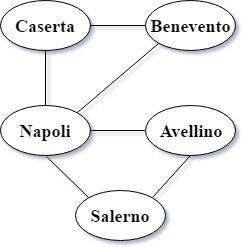
\includegraphics[scale=0.7]{ConstraintGraph.jpg}
		\end{center}
		
		Analizziamo il caso in cui l'agente disponga di solo 2 colori.
		\begin{lstlisting}
Dominio = {Colore1, Colore2}
		\end{lstlisting}
		Applicando il \texttt{Backtracking Search} si perviene presto alla conclusione dell'impossibilità di risolvere il problema vincolato. Ad esempio, applicando le euristiche per migliorare l'efficienza della ricerca, assegniamo a Napoli (\texttt{Degree Heuristic}: variabile con più vincoli sulle rimanenti variabili) il valore Colore1; se procediamo assegnando Colore2 a Caserta (o qualsiasi altra variabile dato che ora presentano tutte un solo valore ammissibile), si ottiene un fallimento, poiché tramite il \texttt{Forward Checking} si osserva che Benevento non può assumere nessun valore ammissibile. Questa risultato è comune anche agli altri path dell'albero di ricerca e tutto ciò è intuitivamente comprensibile poiché con soli 2 colori non siamo in grado di soddisfare i loop di 3 nodi presenti nel grafo dei vincoli.\par
		Analizziamo il caso in cui l'agente disponga di 3 colori.
		\begin{lstlisting}
Dominio = {Colore1, Colore2, Colore3}
		\end{lstlisting}
		Muoviamoci sempre adoperando il solito algoritmo. Partiamo da Napoli assegnandole il Colore1 e notiamo che questa scelta ha ridotto i valori ammisibili per le altre province a due. Coloriamo, ora, Benevento con il Colore2. Caserta sarà la nostra prossima scelta poiché le può essere assegnato solo un colore (abbiamo applicato il \texttt{Minimum Remaining Values}: variabile con numero minimo di valori possibili): essa avrà Colore3. Avellino di conseguenza Colore3 (notiamo che non confina con Caserta e quindi non produce alcun conflitto con la scelta appena fatta), anch'essa con un unico valore possibile, e Salerno, infine, Colore2. Osserviamo che ogni provincia ha un colore diverso dalle confinanti, ma queste ultime  possono essere colorate allo stesso modo nel caso in cui non siano a loro volta adiacenti. Possiamo, in conclusione, affermare che è possibile soddisfare i vincoli dato questo dominio.
		\begin{center}
			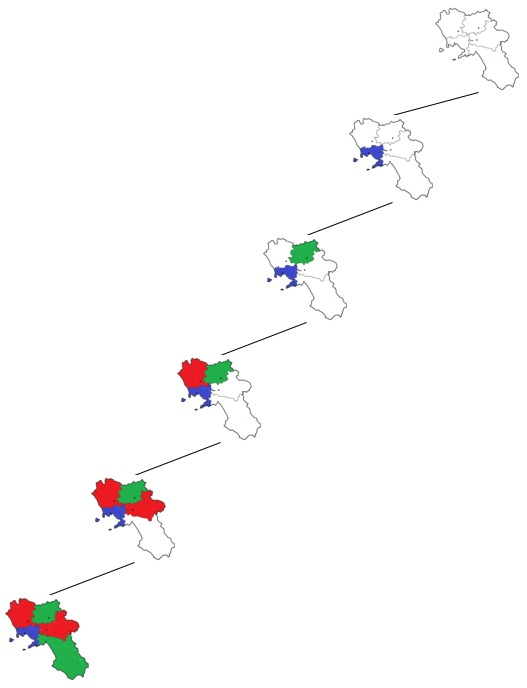
\includegraphics[width=0.6\textwidth, height=0.4\textheight]{SearchTree.jpg}
		\end{center}\par
		Anche il caso con quattro colori sicuramente permetterà di soddisfare i vincoli perché si è aumentato il numero di valori ammissibili lasciando invariate le informazioni iniziali. Verifichiamo che sia così.
		\begin{lstlisting}
Dominio = {Colore1, Colore2, Colore3, Colore4}
		\end{lstlisting}
		La prima provincia che coloriamo è Napoli, assegnandole il Colore1: così facendo riduciamo tutti i colori possibili per le altre province, avendo Napoli il maggior numero di vincoli. Avellino sarà la nostra prossima scelta: assegnandole il Colore2 diminuirà anche il numero di valori per Salerno e Benevento. Passiamo a Caserta: essa può assumere tutti i valori tranne Colore1. Osserviamo, però, che l'assegnazione dei valori Colore3 e Colore4 produrrebbe una diminuzione nei colori sceglibili da Benevento. Applichiamo, allora, il \texttt{Least Constraining Value} (euristica che predilige il valore che lascia più libertà alle variabili adiacenti), optando per Colore2 a Caserta. Segue Benevento con il Colore3 e Salerno con il Colore3. Si noti che, per le ultime due scelte, si può effettuare una scelta completamente arbitraria tra Colore3 e Colore4.\par
		Come ci si poteva aspettare, l'aggiunta di un nuovo elemento nel Dominio, senza l'alterazione dei vincoli, permette ugualmente la risoluzione del problema, perfino evitando di utilizzare il nuovo valore. Possiamo, allora, dedurre che, una volta trovata la soluzione con un determinato numero di valori, essa esisterà anche per un Dominio più esteso. In quest'ultimo caso, però, si può parlare di vincoli più "elastici", più rilassati, grazie ai maggiori gradi di libertà per la determinazione della soluzione. Ad esempio, con un Dominio di tre elementi il numero di soluzioni possibili sicuramente sarà molto più limitato rispetto ad uno con quattro elementi, che permette più opportunità di scelta. Possiamo, quindi, affermare che le soluzioni relative al Dominio esteso includano quelle del Dominio più compatto. 
	\section{Esercizio 4}
		\label{sec:es4}
		Un approccio possibile per trovare la soluzione con l' ausilio di algoritmi genetici potrebbe essere questo:
		Definire come funzione di costo il numero di conflitti, province confinanti con lo stesso colore, il nostro obiettivo è quindi quello di minimizzare questo valore.La popolazione iniziale sarà costituita da delle cartine colorate in modo casuale,dopodiché definiamo una probabilità di mutazione,se non siamo in quest' ultimo caso allora avverrà l' operazione di crossover che consiste nel prendere in modo casuale dall' elite due elementi e scegliere probabilisticamente, quanti cromosomi(province) di uno unire con i restanti dell' altro,altrimenti per la mutazione invece basterà scegliere un elemento dalla cartina e cambiarli colore a scelta tra gli altri tre, escludendo ovviamente quello già assegnato. 
		